% Slides for the talk at HessPL on September 11, 2014.
% http://ps-mr.github.io/hesspl-2014/

\documentclass{beamer}
\usetheme{default}
\setbeamertemplate{navigation symbols}{}
\setbeamertemplate{footline}[frame number]

\usepackage[utf8x]{inputenc}
\usepackage{tikz}
\usetikzlibrary{shapes,arrows,positioning}
\usepackage{verbatim}

\title{A Language for the Specification and Efficient Implementation
  of Type Systems}
\author{Pascal Wittmann}
\institute{TU Darmstadt}
\date{September 11, 2014}

\begin{document}

\begin{frame}[plain]
  \titlepage{}
\end{frame}

\begin{frame}
  \frametitle{Motivation}
  \begin{itemize}
  \item Type systems provide
    \begin{itemize}
    \item static approximation of programs semantics
    \item means to establish and enforce abstraction barriers
    \item documentation that is always correct
    \end{itemize}
  \item Domains specific languages benefit from specialized type
    systems
  \item Gap between formal definitions of type systems and their
    implementations
  \end{itemize}
\end{frame}

\begin{frame}
  \frametitle{Research Problem}
  \begin{itemize}
  \item Design of a declarative specification language that
    \begin{itemize}
    \item is close to text-book formalisms
    \item makes it easy to use existing programming language definitions
    \end{itemize}
  \item Generate first-order formula representations of specifications
  \item Develop a type checker generator which
    \begin{itemize}
    \item is constraint-based
    \item can cope with non-syntax directed rules
    \item takes advantage of facts proven by automated theorem provers
    \end{itemize}
  \end{itemize}
\end{frame}

\begin{frame}[fragile]
  \frametitle{Specification Language}
\begin{verbatim}
module Typesystem

language specifications/SystemF/SystemF

meta-variables 	Term "~" { Type Exp }
                Ctx "$" { TermBinding TypeBinding }
                Id "%" { ID }
                Num "&" { Int }
\end{verbatim}
\end{frame}

\begin{frame}[fragile]
\begin{verbatim}
contexts
TermBinding := ID{I} x Type{O}
TypeBinding := ID{I}

judgments
TermBinding{I} "|" TypeBinding{I} "|-" Exp{I} ":" Type{O}.
Type{O} "= [" ID{I} "->" Type{I} "]" Type{I}.
ID{I} "fresh in" TypeBinding{I}.
ID{I} "!=" ID{I} is Neq.
\end{verbatim}
\end{frame}

\begin{frame}[fragile]
\begin{verbatim}
rules

%x : ~T in $C1        @error %x "should have type" ~T "but has type" INFTYPE.
=============== T-Var
$C1 | $C2 |- %x : ~T

~U = [ %x -> ~S ] ~T            @error ~U "is not" ~T "where" %x "is replaced by" ~S.
$C1 | $C2 |- ~e : all %x . ~T   @error ~e "should have type all" %x "." ~T "but has type" INFTYPE.
============================== T-Tapp
$C1 | $C2 |- ~e [ ~S ] : ~U
\end{verbatim}
\end{frame}

\begin{frame}[fragile]
  \frametitle{Phases of the type checker generator}
\begin{figure}
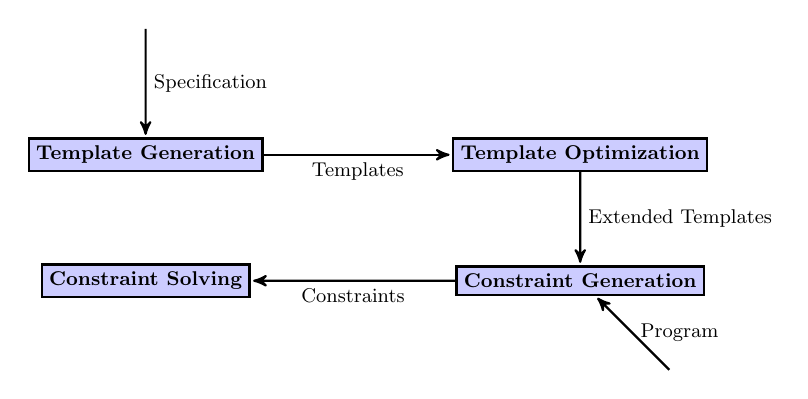
\begin{tikzpicture}[scale=.8,transform shape,->,>=stealth',shorten >=1pt,auto,align=center,node distance=2cm,
  thick,main node/.style={rectangle,fill=blue!20,draw,font=\small\bfseries}]

  \node[main node] (1) {Template Generation};
  \node[main node] (2) [right=3cm of 1] {Template Optimization};
  \node[main node] (3) [below of=2] {Constraint Generation};
  \node[main node] (4) [below of=1] {Constraint Solving};
  \coordinate [below right of=3] (5);
  \coordinate [above of=1] (6);

  \path[every node/.style={font=\small}]
    (1) edge node [right, below] {Templates} (2)
    (2) edge node [right] {Extended Templates} (3)
    (5) edge node [right] {Program} (3)
    (3) edge node [right, below] {Constraints} (4)
    (6) edge node [right] {Specification} (1);
\end{tikzpicture}
\caption{Phases of the type checker generator}
\label{fig:phases}
\end{figure}
\end{frame}

\begin{frame}
  \frametitle{References}
  \bibliographystyle{amsalpha}
  \bibliography{../report/bibliography.bib}
\end{frame}

\end{document}